\chapter{Melody to Tone}
\thispagestyle{empty}

\label{m2t}

{\texttt{2015} -- \texttt{2019}}

\bigskip
\smallskip

\section{Presentation}

This article aims to focus on some tools to interpret a melody to a unique tone with its own identity. The main idea is to analyze an audio sample or a spectrum dataset (generated for instance with the command line \textsl{enkode} with the option \texttt{--spectrum}), with or without the correlated score in order to generate a data profile in terms of `sorting melody' and energy destined to be used as synthesis parameters.

These tools are available in the Common Lisp library named \textsl{cl-gsa}.

\section{Analysis}

\subsection{Segmentation}

Segmentation can be required to extract the harmonic profile or the spectrum of an event of a given sound file. Then the main idea consists to segment the audio file in order to get as many audio files than axiomatic events (notes, chords, or others) forming the melody for analysis.
In practice, it exists some algorithms to realize it, but all use a specific segmentation in a teleological aim, and the relevance is relative. So, each melody will be segmented in an empirical manner with its own tools.

For instance, the command line \textsl{enkode} can realize a segmentation as a TextGrid -- usable with the software Praat -- according to a significative differential loudness and some threshold values defined by the value of the options:
\begin{itemize}
  \item \texttt{--loudness-diff-threshold}
  \item \texttt{--loudness-min-threshold}
  \item \texttt{--loudness-max-threshold}
\end{itemize}

\subsection{Harmonic profile}

The harmonic profile is an ordered list of weight according to the harmonic series. Then the first item is the weight of the root as $f0$, the second item the weight of the first harmonic as $f1$ and so on.

This can be done on one specific sample according to the spectrum analysis of the software Praat and scripted as follow:

\begin{lstlisting}[language=bash]
form Spectrum analysis
    sentence soundfile ...
    positive range ...
endform
Read from file... 'soundfile$'
current_sound$ = selected$ ("Sound")
filedelete 'defaultDirectory$'/'current_sound$'.spectrum
filedelete 'defaultDirectory$'/'current_sound$'.bw
To Spectrum: "yes"  
step=1
repeat 
    res = Get real value in bin: 'step'
    fileappend 'defaultDirectory$'/'current_sound$'.spectrum 'res' 'newline$'
    freq=Get frequency from bin number: 'step'
    step=step+1
until 'freq' > 'range' 	
bw=Get bin width
fileappend 'defaultDirectory$'/'current_sound$'.bw 'bw' 
select all
Remove
\end{lstlisting}

This script generates the \textsl{spectrum} file of the sample and the bandwidth value on the \textsl{bw} file.
Then, the computation of the harmonic profile is done as follow:

\begin{lstlisting}[language=Lisp]
CL-USER> (require 'cl-gsa)
CL-USER> (in-package :cl-gsa)
CL-GSA> (harm-profile (mapcar #'car (read-file 
    "~/piano.spectrum")) 13 (caar (read-file "~/piano.bw")))
Fmax = 984.375 Hz.
Fundamental = 984.375 Hz.
(0.005333674 7.5771334e-4 0.0011644672 1.3338796e-4 7.3244237e-6 7.2097446e-6 2.3828345e-6 4.374403e-6 4.064216e-6 1.18368014e-4 4.6414575e-6 5.292382e-6 2.4746847e-5)

\end{lstlisting}

\begin{figure}[!hbt]
	\begin{center}
		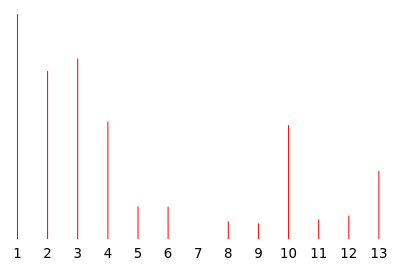
\includegraphics[scale=0.5]{img/4509}
		\caption{Harmonic profile of the piano from a given sample. Note that the graphic representations use a logarithm scale on the y-axis. \mbox{[ $\rightarrow$ \ref{an:pia} ]}}
		\label{fig:piano}
	\end{center}
\end{figure}

\subsection{Sorting melody}

\subsubsection{as harmonic}

The principle is to prioritize the notes of a given melody -- expressed in midi or hertz -- according to their respective harmonics profile as weight list(s) with an approximation set by the nearest division of the whole tone. This is done independently of the melody itself and this depends rather on the number of occurrence of the notes.

The result gives an ordered list of notes according to their importance -- expressed as weight -- in terms of resonance generated by the interaction of their respective harmonics profile according to a deliberate approximation.

\subsubsection{as spectrum}

This can be done also from a spectrum analysis. In this case, the analysis can be done according to the harmonic series fitting the range of the spectrum, or on the whole spectrum by adding all events values by bin.
The result is an ordered bandwidth index as the root harmonics or as the peaks -- or partials -- of the spectral profiles summation.

Here is a short description of the procedure according to the harmonic series:
\begin{itemize}
  \item First, according to the range of the spectrum from 0 to \texttt{*f-range*} (5000 Hz by default) and the number of bins \texttt{*f-bin*} (116 by default) as bandwidth defined by \texttt{*f-range*} divided by \texttt{*f-bin*}, we list all the possible `harmonic' series by bin (done with the function \texttt{all-ser}).
  \item Then, we collect the greater value defined by the summation of the value of each bin width involved divided by the number of bin width involved for each event (done with the function \texttt{mean-sum}).
  \item Then, the summation of all harmonic series selected, by column (in another word by bin) is done with the function \texttt{summation-hors-tps}. The result is the weighted `sorting melody' according to the indices of the frequency bandwidth.
\end{itemize}

Thus, the melodic profile of the sample is estimated according to the sorting melody as indices of frequency bandwidth.

\bigskip 

The spectrum analysis can be done for each event of a sound file with the command line \textsl{enkode} according to the values defined by the options \texttt{-spectrum} and \texttt{--smooth-frequency}.

\subsection{Energy profile}

Now it exists a powerful tool called \texttt{energy-prof-morph-analysis} -- renamed \texttt{energy-profile} in \textsl{cl-gsa} -- from the library Morphologie developed at the IRCAM \citep{mp}. The function \texttt{energy-prof-morph-analysis} is applied on the result of the function \texttt{new-old-analysis} which is described in the article \textit{Morphological Analysis} \citep{ma}.

\bigskip 

However, to resume and for the record, let illustrate these algorithmic processes with the following sorting melody as the symbolic list \texttt{(a b c b d e f)} for instance.

The first step is to realize the analysis of contrast described in the Paolo Aralla's article [op. cit.].

\bigskip

\begin{quotation} 
\begin{slshape} 
\noindent The analysis of contrasts, which is the function at heart of the Morphologie Library developed by Jacopo Baboni Schilingi and Frederic Voisin, identifies the occurrences within any sequence of events.

\noindent Such analysis is of quantitative type, and has considerable development potentialities towards a qualitative description of the processes that put in relation morphologic structure of the message, mnemonic perceptive activity and psychic response.

\noindent The hierarchies that the analysis of contrasts describes become qualitatively pertinent to the mnemonic activity.

\noindent We have called New/Old Analysis the function that describes the newness level of an event in relation to the context in which it appears.

\noindent The importance of such a function is crucial, because it describes from the point of view of the psychic response the different newness level of the single event in the time.

\noindent The steps to define New/Old Analysis are three:

\noindent 1 - Measurement of the distances:

\pagebreak

\noindent it allows to quantify the local distance between the different events in relation to their first appearance in the time.
\end{slshape}

\noindent\texttt{\footnotesize (defun distances (sequence)}

\noindent\texttt{\footnotesize \quad  (mapcar \#' (lambda (x) (x->dx x)) (Contrasts-all-lev sequence)))}

\begin{quotation} 
\begin{slshape} 
\noindent The Analysis of the Contrasts, formulated by Herv\'e Rivi\`ere and Fr\'ed\'eric Voisin, and implemented in the OpenMusic Morphologie Library, is a model able to describe the becoming of the form in the time.

\noindent It points out the hierarchic relation created by the temporal sequence of the events: in fact, for the mnemonic activity, each event is datum point for every following event and datum point for the previous ones.

\noindent The numerical transcription carried out through the Analysis of Contrasts describes the entry order of the events in the time.

\noindent We could define the numerical transcription created using the analysis of contrasts as morphological structure of the entry order of the events.

\noindent From this starting point it is possible to identify the presence of internal patterns and analyse their potential capacity to describe and re-establish the form in its original status.

\noindent exemple:
\end{slshape}

\noindent\texttt{\footnotesize (contrasts-all-lev '(a d f g f)) ----> ((1 2 3 4 3) (1 2 3 2) (1 2 1) (1 2))}

\noindent (Documentation of \texttt{contrasts-all-lev})
\end{quotation} 
\begin{slshape} 
\noindent 2. Attribution of different weights to the datum points:

\noindent this step is crucial, because it strengthens the global hierarchy among the various analysis level in relation to the time parameter.
\end{slshape} 

\noindent\texttt{\footnotesize (defun weights (sequence)}

\noindent\texttt{\footnotesize \quad   (mapcar \#' (lambda (x) (apply '+ x))}

\noindent\texttt{\footnotesize \quad \quad  (Contrasts-all-lev sequence)))}

\begin{slshape} 
\noindent 3. Application of weights to the distances:

\noindent this further step is just the application of different weights - obtained considering every time one of the events as datum point (global parameter, ex. nr. 3) - to the distances between the various contiguous events (local parameter).
\end{slshape} 

\noindent\texttt{\footnotesize (defun Contrasts-lev.1*weights (sequence)}

\noindent\texttt{\footnotesize \quad    (mapcar \#' (lambda (x y) (om* y x))}

\noindent\texttt{\footnotesize \quad  \quad (distances sequence) (weights sequence)))}

\noindent\texttt{\footnotesize ;--------}

\noindent\texttt{\footnotesize (defun Contrasts-all-lev*weights (sequence)}

\noindent\texttt{\footnotesize \quad   (reverse (mapcar \#' (lambda (xx) (apply '+ xx))}

\noindent\texttt{\footnotesize \quad \quad (mat-trans (mapcar \#' (lambda (x) (reverse x)) (Contrasts-lev.1 *}

\noindent\texttt{\footnotesize \quad \quad \quad weights sequence))))))}

\begin{slshape} 
\noindent A theoretical problem we have faced is the relation between the object we have analyzed and the previous and following events. Any events chain perceived as belonging to a whole and complete organism stays anyway in relation with the previous and following sequential chain.

\noindent In case of performance of a music piece, the silence acts as a frame of the structure, and, being a frame, it becomes an organic element of the structure analyzed.

\noindent It is worth to underline that even in case of extrapolation, like in the here quoted examples (a thematic fragment, a subject of a fugue, etc.), the object is perceived as a unit, and therefore the silence places it in a well defined mental space.
\end{slshape}

\noindent (Documentation of \texttt{new-old-analysis})
\end{quotation} 

\noindent \texttt{\textbf{*start*}} = symbol-silence-start

\noindent \texttt{\textbf{*stop*}} = symbol-silence-end

\begin{center}
\begin{tabular}{cccccccccc}
  \cellcolor {gray!20} \texttt{\textbf{*start*}} & \cellcolor {gray!20} \texttt{a} & \cellcolor {gray!20} \texttt{b} & \cellcolor {gray!20} \texttt{c} & \cellcolor {gray!20} \texttt{b} & \cellcolor {gray!20} \texttt{d} & \cellcolor {gray!20} \texttt{e} & \cellcolor {gray!20} \texttt{f} & \cellcolor {gray!20} \texttt{\textbf{*stop*}} & \\
  1 & 2 & 3 & 4 & 3 & 5 & 6 & 7 & 8 & \cellcolor {gray!20} \bf 39 \\
    & 1 & 2 & 3 & 2 & 4 & 5 & 6 & 7 & \cellcolor {gray!20} \bf 30 \\
    &   & 1 & 2 & 1 & 3 & 4 & 5 & 6 & \cellcolor {gray!20} \bf 22 \\
    &   &   & 1 & 2 & 3 & 4 & 5 & 6 & \cellcolor {gray!20} \bf 21 \\
    &   &   &   & 1 & 2 & 3 & 4 & 5 & \cellcolor {gray!20} \bf 15 \\   
    &   &   &   &   & 1 & 2 & 3 & 4 & \cellcolor {gray!20} \bf 10 \\   
    &   &   &   &   &   & 1 & 2 & 3 & \cellcolor {gray!20} \bf 6 \\    
    &   &   &   &   &   &   & 1 & 2 & \cellcolor {gray!20} \bf 3 \\      
\end{tabular}
\end{center}

\bigskip 

Then we get all $dx$ by row which will be multiplied by the previous summation.

\begin{center}
\begin{tabular}{ccccccccc}
\quad 1 \quad & \quad 1 \quad & \quad 1 \quad & \quad -1 \quad & \quad 2 \quad & \quad 1 \quad & \quad 1 \quad & \quad 1 \quad & \cellcolor {gray!20} \bf 39 \\
 \quad \quad & \quad 1 \quad & \quad 1 \quad & \quad -1 \quad & \quad 2 \quad & \quad 1 \quad & \quad 1 \quad & \quad 1 \quad & \cellcolor {gray!20} \bf 30 \\
 \quad \quad & \quad \quad & \quad 1 \quad & \quad -1 \quad & \quad 2 \quad & \quad 1 \quad & \quad 1 \quad & \quad 1 \quad & \cellcolor {gray!20} \bf 22 \\
 \quad \quad & \quad \quad & \quad \quad & \quad 1 \quad & \quad 1 \quad & \quad 1 \quad & \quad 1 \quad & \quad 1 \quad & \cellcolor {gray!20} \bf 21 \\
 \quad \quad & \quad \quad & \quad \quad & \quad \quad & \quad 1 \quad & \quad 1 \quad & \quad 1 \quad & \quad 1 \quad & \cellcolor {gray!20} \bf 15 \\ 
 \quad \quad & \quad \quad & \quad \quad & \quad \quad & \quad \quad & \quad 1 \quad & \quad 1 \quad & \quad 1 \quad & \cellcolor {gray!20} \bf 10 \\ 
 \quad \quad & \quad \quad & \quad \quad & \quad \quad & \quad \quad & \quad \quad & \quad 1 \quad & \quad 1 \quad & \cellcolor {gray!20} \bf 6 \\ 
 \quad \quad & \quad \quad & \quad \quad & \quad \quad & \quad \quad & \quad \quad & \quad \quad & \quad 1 \quad & \cellcolor {gray!20} \bf 3 \\
\end{tabular}
\end{center}

\bigskip 

Then we make the sum of each column.

\begin{center}
\begin{tabular}{cccccccc}
39 & 39 & 39 & -39 & 78	& 39 & 39 & 39 \\
   & 30 & 30 & -30 & 60 & 30 & 30 & 30 \\
   & 	& 22 & -22 & 22 & 22 & 22 & 22 \\
   &    &    &  21 & 21 & 21 & 21 & 21 \\
   &    &    &     & 15 & 15 & 15 & 15 \\
   &    &    &     &    & 10 & 10 & 10 \\
   &    &    &     &    &    &	6 & 6 \\
   &    &    &     &    &    &    & 3 \\
\cellcolor {gray!20} \bf 39 & \cellcolor {gray!20} \bf 69 & \cellcolor {gray!20} \bf 91 & \cellcolor {gray!20} \bf -70	& \cellcolor {gray!20} \bf 218 & \cellcolor {gray!20} \bf 137	& \cellcolor {gray!20} \bf 143 & \cellcolor {gray!20} \bf 146\\
\end{tabular}
\end{center}

\bigskip 

This `temporary' result \texttt{(39 69 91 -70 218 137 143 146)} corresponds to the analysis of contrasts called \texttt{new-old-analysis} in the Morphologie library.

\begin{quotation} 
\begin{slshape} 
\noindent The step that allows transforming the new-old-analysis function into a model able to simulate the psychic response of the perceptive act to the morphologic structure occurs using three functions.

\noindent Then, to this, the three functions apply to allow to define the energy profile.

\noindent 1. In the first passage, the transformation into absolute abs value contains all the relations with reference to the first element of the chain.

\noindent At this point, the data do not represent the ageing degree of the events anymore, but they are mere distance (it does not matter if they are old or new, they are to be intended nearly as physical distance between the various data stored in space/memory) related to a virtual point zero (a kind of possible present)

\noindent 2. In the second passage, the use of the local derivative, implemented in OpenMusic under the name of x–>dx, the contiguous relations are again pointed out, and the distance identified in the first passage is assimilated to the energy needed to cover the contiguous distances in space/memory

\noindent 3. Finally, the transformation into absolute abs value, because of the transformation of the distances into energy, brings all the data back to positive values.
\end{slshape} 

\noindent (Documentation of \texttt{energy-prof-morph-analysis})
\end{quotation} 

\bigskip

\noindent
\begin{adjustbox}{center}
\begin{tabular}{cccccccccccccccc}
 &	0 &	 &	39 & &	69 & &	91 & &	-70 & &	218 & &	137 & &	143 \\
\cellcolor {gray!20} $abs$ & 0 & &	39 & & 69 & & 91 & & 70 & &	218 & &	137 & &	143 \\
\cellcolor {gray!20} $x \rightarrow dx$ & & 39 & &	30 & & 22 & & -21 & & 148 & & -81 & & 6 & \\
\cellcolor {gray!20} $abs$ &\cellcolor {gray!20} &\cellcolor {gray!20} \bf 39 &\cellcolor {gray!20} &\cellcolor {gray!20} \bf 30 &\cellcolor {gray!20} &\cellcolor {gray!20} \bf 22 &\cellcolor {gray!20} &\cellcolor {gray!20} \bf 21 &\cellcolor {gray!20} &\cellcolor {gray!20} \bf 148 &\cellcolor {gray!20} &\cellcolor {gray!20} \bf 81 &\cellcolor {gray!20} &\cellcolor {gray!20} \bf 6 &\cellcolor {gray!20} \\
\end{tabular}
\end{adjustbox}

\bigskip 

Note that this kind of analysis is strictly symbolic, focusing the structure of contrast, and all symbols of the list are initially only referred to themselves. In our case, symbols can refer to the pitches, intervals, durations, along with others.

\section{Instantiation}

The library \textsl{cl-gsa} allows three types of data: \texttt{:midi} as a list of midi notes or as a list of chords as list of midi notes; \texttt{:freq} as a list of frequencies or as a list of clusters as list of frequencies; \texttt{:spectrum} as a list of spectrum profiles defined as events.

The sorting melody and the energy profile can be used independently according to the modalities of the user. The main function \texttt{m2tab} allows to compute both at the same time and optionally offers the possibility to write the result in a file defined by its path.

\subsection{From a partition}

For instance, according to the partition of figure \ref{fig:op11}, the sorting melody and the energy profile is done according to the following steps:

\begin{figure}[!hbt]
	\begin{center}
		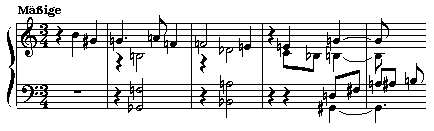
\includegraphics[scale=0.6]{img/2311}
		\caption{Arnold Schoenberg: opening phrase of \textit{Drei Klavierstucke} for solo piano, opus 11.}
		\label{fig:op11}
	\end{center}
\end{figure}

\begin{enumerate}
\item 
Convert the partition to a midi score according the following syntax:
\begin{lstlisting}[language=Lisp]
CL-GSA> (defparameter *score* '((71) (68) (67) (59 53 42) (69) (65) (65) (61 57 46) (64) (60 64) (58) (67 59 50 42) (54) (57) (58) (59)))
\end{lstlisting}

\item
The harmonic profile is given by the computation done in figure \ref{fig:piano}.

\begin{lstlisting}[language=Lisp]
CL-GSA> (defparameter *harmonic-profile-piano* '(0.005333674  7.5771334e-4  0.0011644672 1.3338796e-4 7.3244237e-6  7.2097446e-6  2.3828345e-6  4.374403e-6 4.064216e-6  1.18368014e-4  4.6414575e-6  5.292382e-6 2.4746847e-5))
\end{lstlisting}

\item
Then, the main function \texttt{m2tab} display the result with by line the frequency of the note involves in the initial melody, the weight of the sorting melody (or in other words the energy of the signal), the weight of the energy profile as the `formal' energy and the midi note. The last argument allows to write the result according to a given path name.   

\begin{lstlisting}[language=Lisp]
CL-GSA> (m2tab (sort-melody :midi *score* :harm-weight
   *harmonic-profile-piano* :approx 8) "~/test")
246.94165   0.11377126      0.087647595     59.0
349.22824   0.0894084       0.0849228       65.0
92.498604   0.08421194      0.014191644     42.0
233.08186   0.08116744      0.20640327      58.0
220.0       0.07584624      0.09196185      57.0
...
\end{lstlisting}

The approximation concerns the accuracy of the harmonic match.
\end{enumerate}

\subsection{From a sound file}

It is possible to work directly from a sound file. The command line \textsl{enkode} with the option \texttt{--spectrum} allows to segment the sample as spectrum events list, which can be used either as harmonic or as spectrum in order to compute the sorting melody and the energy profile. 

\begin{enumerate}
\item
Segment the sound file with \textsl{enkode}:
\begin{lstlisting}[language=bash]
$ enkode --spectrum --loudness-diff-thres=1.48 test.mp3 > test.spectrum
\end{lstlisting}

\item
Then, the main function \texttt{m2tab} display the result with by line the top frequency as the indice multiply by the bandwidth value (5000/116 in this case), the `presence' as the energy of the signal, the `formal' energy and the index of the salient frequency bandwidth.   
\begin{lstlisting}[language=Lisp]
CL-GSA> (m2tab (sort-melody :spectrum (read-file 
   "~/test.spectrum") :partial 3) "~/test")
387.93103   0.4931115       0.022011383     8
344.82758   0.20561041      0.020645158     7
431.0345    0.11075174      0.05981024      9
1508.6206   0.03852629      0.03248577      34
1594.8275   0.021509826     0.039165083     36
...
\end{lstlisting}
\end{enumerate}

\section{Synthesis}

The synthesizer I chose reproduces the `sustain' of a piano. I scaled the level from 0.01 to 0.1 and the energy (that I transposed in term of `grain' that is to say a kind of `texturation') from 300 to 3000 Hz. The synthesis is realized with the software SuperCollider.
\newpage
\begin{lstlisting}[language=Java]
// inspired by the synthetic piano patch (James McCartney) originally for SC2, 1998.
(
SynthDef(\op11M2T, { |bus=0, pitch=60, amp=0.1, grain=3000|
	var detune, delayTime, noise, out;
	out = Mix.ar(Array.fill(3, { arg i;
		// detune strings, calculate delay time :
		detune = #[-0.05, 0, 0.04].at(i);
		delayTime = 1 / (pitch + detune).midicps;
		// each string gets own exciter :
		noise = LFNoise2.ar(grain, 0.1); // grain = 3000 Hz is the reference
		CombL.ar(noise,		
		// used as a string resonator
			delayTime, 	
			// max delay time
			delayTime,	
			// actual delay time
			6
			// decay time of string
			)
	}));
	Out.ar(bus, Splay.ar(out*amp)*EnvGen.ar(Env.linen(0.5,10,3.0),doneAction:2))}).add
)

~data = FileReader.read("~/test.m2t".standardizePath).collect({|line| line.collect({|val| val.asFloat})}) 
 
(instrument: \resPiano, pitch: ~data.flop[0].cpsmidi, amp:
   ~data.flop[1].normalize(0.01, 0.1), grain: 
   ~data.flop[2].normalize(300, 3000)).play;
\end{lstlisting}

\section{Discussion}

I exposed the basics of some \textsl{cl-gsa} tools in the context of `converting' a melody to an unique tone (M2T) as timbre. And of course, the possibilities of interpretation are infinite, but these tools allow managing this kind of transposition -- that is to say the `transformation' of a melody to a unique tone -- with relevance and open a substantial field of creativity.

In any case, this process is destructive in a way that it is not possible to retrieve the original melody from the tone profile. In other words, a melody has one tone profile according to one process, and a tone profile with the same process can be generated with different melodies.